% answers.tex —— 2000 年·春季京皖卷·文科 · 参考答案与详细解析片段
% 由 tools/generate_projects.py 依来源总账自 2000/2000_数学真题_春季京皖文_试题.md + 2000/2000_数学真题_春季京皖文_解析正文.md + 2000/2000_数学真题_春季京皖文_答案要点.md 生成，勿手改（改源 MD 后重跑）


\begin{gknotice}
\textbf{解析归属}：固定源 PDF 只有题面，没有答案页。以下推导依据固定题面形成，\textbf{非官方解析}；已由独立解题者在只读题面条件下盲解（24 题），转录另经 300 dpi 与内容流核对。源内疑点保留在题面与答案要点中，不以推导结果反改原题。
\end{gknotice}

\begin{answer}
\gksolhead{1}{}

\textbf{题目}：

复数 $z_1 = 3 + \mathrm{i}$，$z_2 = 1 - \mathrm{i}$，则 $z = z_1 \cdot z_2$ 在复平面内的对应点位于　（　）

（A）第一象限　（B）第二象限　（C）第三象限　（D）第四象限

\Needspace{4\baselineskip}
\textbf{解析}

$z=z_1z_2=(3+\mathrm i)(1-\mathrm i)=3-3\mathrm i+\mathrm i-\mathrm i^2=4-2\mathrm i$，对应点 $(4,-2)$，实部 $>0$、虚部 $<0$，位于第四象限。

验证：$|z|=|z_1||z_2|=\sqrt{10}\cdot\sqrt2=2\sqrt5$，而 $|4-2\mathrm i|=\sqrt{16+4}=2\sqrt5$，模一致；辐角 $=\arctan(-1/2)$ 在第四象限，与坐标位置相符。

\gkanswer{答案：D}

\end{answer}
\begin{answer}
\gksolhead{2}{}

\textbf{题目}：

设全集 $I = \{a, b, c, d, e\}$，集合 $M = \{a, c, d\}$，$N = \{b, d, e\}$，那么 $\overline{M} \cap \overline{N}$ 是　（　）

（A）$\varnothing$　（B）$\{d\}$　（C）$\{a, c\}$　（D）$\{b, e\}$

\Needspace{4\baselineskip}
\textbf{解析}

$\overline M=\{b,e\}$，$\overline N=\{a,c\}$，故 $\overline M\cap\overline N=\{b,e\}\cap\{a,c\}=\varnothing$。亦可由 $\overline M\cap\overline N=\overline{M\cup N}$，而 $M\cup N=\{a,b,c,d,e\}=I$，补集为空集。

验证：$M\cup N=\{a,b,c,d,e\}=I$，$\overline I=\varnothing$，与直接求交结果一致；且 $M\cap N=\{d\}$ 恰为选项 (B)，说明命题人以此作干扰项，逻辑自洽。

\gkanswer{答案：A}

\end{answer}
\begin{answer}
\gksolhead{3}{}

\textbf{题目}：

已知双曲线 $\frac{x^2}{b^2} - \frac{y^2}{a^2} = 1$ 的两条渐近线互相垂直，那么该双曲线的离心率是　（　）

（A）$2$　（B）$\sqrt{3}$　（C）$\sqrt{2}$　（D）$\frac{3}{2}$

\Needspace{4\baselineskip}
\textbf{解析}

双曲线 $\dfrac{x^2}{b^2}-\dfrac{y^2}{a^2}=1$ 的渐近线为 $y=\pm\dfrac{a}{b}x$。两渐近线互相垂直 $\iff$ 两斜率之积 $-\dfrac{a^2}{b^2}=-1\iff a=b$。于是 $c=\sqrt{a^2+b^2}=\sqrt2\,b$，离心率 $e=\dfrac{c}{b}=\sqrt2$。

验证：取 $a=b=1$ 得 $x^2-y^2=1$，渐近线 $y=\pm x$ 互相垂直 ，$e=c/a_{\text{\text{实}}}=\sqrt2$ 。若 $a\ne b$ 则 $-\frac{a^2}{b^2}\ne-1$，垂直不成立，说明条件与结论等价。

\gkanswer{答案：C}

\end{answer}
\begin{answer}
\gksolhead{4}{}

\textbf{题目}：

下列方程关于 $x = y$ 对称的是　（　）

（A）$x^2 - x + y^2 = 1$　（B）$x^2 y + x y^2 = 1$

（C）$x - y = 1$　（D）$x^2 - y^2 = 1$

\Needspace{4\baselineskip}
\textbf{解析}

曲线关于 $y=x$ 对称 $\iff$ 方程在 $x,y$ 互换后不变。
(A) $x^2-x+y^2=1\to y^2-y+x^2=1$，改变；(B) $x^2y+xy^2=1\to y^2x+yx^2=1$，不变 ；(C) $x-y=1\to y-x=1$，改变；(D) $x^2-y^2=1\to y^2-x^2=1$，改变。

验证：取 (B) 上一点：令 $x=1$，$y^2+y-1=0$ 得 $y=\frac{\sqrt5-1}{2}\approx0.618$。互换后的点 $(0.618,1)$ 代入 $x^2y+xy^2=0.382\times1+0.618\times1=1$ ，仍在曲线上。

\gkanswer{答案：B}

\end{answer}
\begin{answer}
\gksolhead{5}{}

\textbf{题目}：

一个圆锥的底面直径和高都同一个球的直径相等，那么圆锥与球的体积之比是　（　）

（A）$1:3$　（B）$2:3$　（C）$1:2$　（D）$2:9$

\Needspace{4\baselineskip}
\textbf{解析}

设球半径 $R$，则球直径 $2R$。圆锥底面直径 $=2R$，故底半径 $r=R$；高 $h=2R$。
$V_{\text{\text{锥}}}=\frac13\pi R^2\cdot 2R=\frac23\pi R^3$，$V_{\text{\text{球}}}=\frac43\pi R^3$，比值 $\frac23:\frac43=1:2$。

验证：令 $R=1$：$V_{\text{\text{锥}}}=\frac13\pi\cdot1^2\cdot2=2.094$，$V_{\text{\text{球}}}=\frac43\pi=4.189$，比值 $0.5=1:2$ 。量纲上两体积同为 $R^3$ 的量级，比值必为纯数，与 $R$ 无关 。

\gkanswer{答案：C}

\end{answer}
\begin{answer}
\gksolhead{6}{}

\textbf{题目}：

直线 $(\sqrt{3} - \sqrt{2})x + y = 3$ 和直线 $x + (\sqrt{2} - \sqrt{3})y = 2$ 的位置关系是　（　）

（A）相交但不垂直　（B）垂直　（C）平行　（D）重合

\Needspace{4\baselineskip}
\textbf{解析}

$l_1$：$y=(\sqrt2-\sqrt3)x+3$，$k_1=\sqrt2-\sqrt3$；$l_2$：$(\sqrt2-\sqrt3)y=2-x$，$k_2=\dfrac{-1}{\sqrt2-\sqrt3}$。
$k_1k_2=(\sqrt2-\sqrt3)\cdot\dfrac{-1}{\sqrt2-\sqrt3}=-1$，故两直线垂直。

验证：取两直线的法向量：$l_1$ 的法向量为 $(\sqrt3-\sqrt2,\,1)$，$l_2$ 的法向量为 $(1,\,\sqrt2-\sqrt3)$，内积 $=(\sqrt3-\sqrt2)+(\sqrt2-\sqrt3)=0$ ，法向量垂直即直线垂直。

\gkanswer{答案：B}

\end{answer}
\begin{answer}
\gksolhead{7}{}

\textbf{题目}：

函数 $y = \lg |x|$　（　）

（A）是偶函数，在区间 $(-\infty, 0)$ 上单调递增

（B）是偶函数，在区间 $(-\infty, 0)$ 上单调递减

（C）是奇函数，在区间 $(0, +\infty)$ 上单调递增

（D）是奇函数，在区间 $(0, +\infty)$ 上单调递减

\Needspace{4\baselineskip}
\textbf{解析}

定义域 $x\ne0$ 关于原点对称，$f(-x)=\lg|-x|=\lg|x|=f(x)$，故为偶函数。
当 $x<0$ 时 $f(x)=\lg(-x)$，内层 $u=-x$ 随 $x$ 增大而减小，而 $\lg u$ 单增，故 $f$ 在 $(-\infty,0)$ 上单调递减。

验证：$f(-10)=\lg10=1$，$f(-1)=\lg1=0$，$x$ 由 $-10$ 增到 $-1$ 时函数值由 $1$ 降到 $0$，递减 （与 (A) 相反）。

\gkanswer{答案：B}

\end{answer}
\begin{answer}
\gksolhead{8}{}

\textbf{题目}：

从单词“equation”选取 5 个不同的字母排成一排，含有“qu”（其中“qu”相连且顺序不变）的不同排列共有　（　）

（A）120 个　（B）480 个　（C）720 个　（D）840 个

\Needspace{4\baselineskip}
\textbf{解析}

"equation" 的 8 个字母 $e,q,u,a,t,i,o,n$ 互不相同。把 "qu" 捆绑成一个元素（顺序固定），则还需从其余 6 个字母中选 3 个：$\mathrm C_6^3=20$ 种。将 "qu" 块与这 3 个字母共 4 个元素全排列：$4!=24$。共 $20\times24=480$。

验证：换一条路径：含 $q,u$ 的 5 字母排列共 $\mathrm C_6^3\cdot5!=2400$ 种，其中 $q$ 恰在 $u$ 前一位的占 $4!/5!=1/5$，得 $2400/5=480$ 。

\gkanswer{答案：B}

\end{answer}
\begin{answer}
\gksolhead{9}{}

\textbf{题目}：

椭圆短轴长是 2，长轴长是短轴的 2 倍，则椭圆中心到其准线距离是　（　）

（A）$\frac{8}{5}\sqrt{5}$　（B）$\frac{4}{5}\sqrt{5}$　（C）$\frac{8}{3}\sqrt{3}$　（D）$\frac{4}{3}\sqrt{3}$

\Needspace{4\baselineskip}
\textbf{解析}

短轴长 $2b=2\Rightarrow b=1$；长轴长 $=2\times$短轴长 $=4\Rightarrow a=2$。$c=\sqrt{a^2-b^2}=\sqrt3$。
中心到准线距离 $=\dfrac{a^2}{c}=\dfrac{4}{\sqrt3}=\dfrac{4\sqrt3}{3}$。

验证：准线 $x=\pm\frac{a^2}{c}=\pm2.309$，中心到准线距离 $2.309=\frac{4\sqrt3}{3}$ ；又 $\frac{a^2}{c}=\frac{4}{1.732}=2.309>a=2$，准线在顶点之外，符合椭圆性质。

\gkanswer{答案：D}

\end{answer}
\begin{answer}
\gksolhead{10}{}

\textbf{题目}：

函数 $y = \sin x + \cos x + 2$ 的最小值是　（　）

（A）$2 - \sqrt{2}$　（B）$2 + \sqrt{2}$　（C）$0$　（D）$1$

\Needspace{4\baselineskip}
\textbf{解析}

$\sin x+\cos x=\sqrt2\sin\!\left(x+\frac\pi4\right)\in[-\sqrt2,\sqrt2]$，故 $y_{\min}=2-\sqrt2$，在 $\sin(x+\frac\pi4)=-1$ 即 $x=-\frac{3\pi}{4}+2k\pi$ 处取到。

验证：取 $x=-\frac{3\pi}{4}$：$\sin x=-\frac{\sqrt2}{2}$，$\cos x=-\frac{\sqrt2}{2}$，$y=2-\sqrt2\approx0.586$ ；取 $x=\frac{\pi}{4}$ 得 $y=2+\sqrt2$（最大值），与 (B) 对应，说明两选项互为最大/最小值，配对合理。

\gkanswer{答案：A}

\end{answer}
\begin{answer}
\gksolhead{11}{}

\textbf{题目}：

设复数 $z_1 = -1 - \mathrm{i}$ 在复平面上对应向量 $\overrightarrow{OZ_1}$，将 $\overrightarrow{OZ_1}$ 按顺时针方向旋转 $\frac{5}{6}\pi$ 后得到向量 $\overrightarrow{OZ_2}$，令 $\overrightarrow{OZ_2}$ 对应的复数为 $z_2$ 的辐角主值为 $\theta$，则 $\tan\theta =$　（　）

（A）$2 - \sqrt{3}$　（B）$-2 + \sqrt{3}$　（C）$2 + \sqrt{3}$　（D）$-2 - \sqrt{3}$

\Needspace{4\baselineskip}
\textbf{解析}

$z_1=-1-\mathrm i$ 的辐角为 $225^\circ$。顺时针旋转 $\frac56\pi=150^\circ$ 后辐角为 $225^\circ-150^\circ=75^\circ\in(0^\circ,90^\circ)$，即主值 $\theta=75^\circ$。
$\tan75^\circ=\tan(45^\circ+30^\circ)=\dfrac{1+\frac{\sqrt3}{3}}{1-\frac{\sqrt3}{3}}=\dfrac{3+\sqrt3}{3-\sqrt3}=2+\sqrt3$。

验证：直接相乘：$z_2=z_1\mathrm e^{-\mathrm i\frac{5\pi}{6}}=(-1-\mathrm i)\left(-\frac{\sqrt3}{2}-\frac{\mathrm i}{2}\right)=\frac{\sqrt3-1}{2}+\mathrm i\,\frac{1+\sqrt3}{2}$，实虚部均为正（第一象限，$75^\circ$ ），$\tan\theta=\frac{1+\sqrt3}{\sqrt3-1}=2+\sqrt3$ 。若误按逆时针则得 $\tan15^\circ=2-\sqrt3$，对应干扰项 (A)。

\gkanswer{答案：C}

\end{answer}
\begin{answer}
\gksolhead{12}{}

\textbf{题目}：

设 $\alpha$，$\beta$ 是一个钝角三角形的两个锐角，下列四个不等式中不正确的是　（　）

（A）$\tan\alpha \tan\beta < 1$　（B）$\sin\alpha + \sin\beta < \sqrt{2}$

（C）$\cos\alpha + \cos\beta > 1$　（D）$\frac{1}{2}\tan(\alpha+\beta) < \tan\frac{\alpha+\beta}{2}$

\Needspace{4\baselineskip}
\textbf{解析}

钝角三角形中两锐角 $\alpha,\beta\in(0,\frac\pi2)$ 且 $s=\alpha+\beta<90^\circ$。
(A) $\tan s=\dfrac{\tan\alpha+\tan\beta}{1-\tan\alpha\tan\beta}>0$，分子为正，故分母 $1-\tan\alpha\tan\beta>0$，即 $\tan\alpha\tan\beta<1$，正确。
(B) $\sin\alpha+\sin\beta=2\sin\frac s2\cos\frac{\alpha-\beta}{2}\le2\sin\frac s2<2\sin45^\circ=\sqrt2$，正确。
(C) $\cos\alpha+\cos\beta=2\cos\frac s2\cos\frac{\alpha-\beta}{2}\ge2\cos^2\frac s2=1+\cos s>1$，正确。
(D) 令 $t=\frac{\alpha+\beta}{2}\in(0,45^\circ)$，则 $0<\tan t<1$，$\frac12\tan(2t)=\dfrac{\tan t}{1-\tan^2 t}>\tan t$，所给不等式\textbf{不成立}。

验证：取 $\alpha=\beta=30^\circ$（$s=60^\circ<90^\circ$）：$\tan\alpha\tan\beta=\frac13<1$ ；$\sin\alpha+\sin\beta=1<\sqrt2$ ；$\cos\alpha+\cos\beta=\sqrt3\approx1.732>1$ ；而 $\frac12\tan60^\circ\approx0.866>\tan30^\circ\approx0.577$，(D) 的 "<" 方向反了 。

\gkanswer{答案：D}

\end{answer}
\begin{answer}
\gksolhead{13}{}

\textbf{题目}：

已知等差数列 $\{a_n\}$ 满足 $a_1 + a_2 + a_3 + \cdots + a_{101} = 0$，则有　（　）

（A）$a_1 + a_{101} > 0$　（B）$a_2 + a_{100} < 0$　（C）$a_3 + a_{99} = 0$　（D）$a_{51} = 51$

\Needspace{4\baselineskip}
\textbf{解析}

$S_{101}=\dfrac{101(a_1+a_{101})}{2}=0\Rightarrow a_1+a_{101}=0\Rightarrow 2a_{51}=0\Rightarrow a_{51}=0$。
于是 $a_3+a_{99}=2a_{51}=0$。其余：(A) $a_1+a_{101}=0$ 不 $>0$；(B) $a_2+a_{100}=2a_{51}=0$ 不 $<0$；(D) $a_{51}=0\ne51$。

验证：取 $a_n=(n-51)k$（公差 $k$），则 $S_{101}=101a_{51}=0$ ；$a_3+a_{99}=(3-51)k+(99-51)k=-48k+48k=0$ 。

\gkanswer{答案：C}

\end{answer}
\begin{answer}
\gksolhead{14}{}

\textbf{题目}：

已知函数 $f(x) = ax^3 + bx^2 + cx + d$ 的图象如图，则　（　）
\nopagebreak[4]
\begin{center}% ============================================================================
% 2000 年春季高考（京、皖）文科 第 14 题：三次函数 y = f(x) 的图象
% ----------------------------------------------------------------------------
% 来源：.work/phase4-b20/source/2000春季京皖文.pdf
%       SHA-256 b9552b8354735296f6ea1ed051085e094e4af0c14ff97ada2dbd4e579b14287f
%       第 1 页，内容流对象 39 / 40 / 42 / 43 / 44 / 45 / 46 / 47（按页面资源顺序拼接解析）
% 重绘方式：qpdf --qdf 取内容流 → 解析 m/l/c/re/S/f、w、d → 本地坐标
%          本地坐标 = 页面坐标 − (608.528, 616.430)，原点取坐标轴交点 O；
%          1 单位 = 1 TeX pt；页面为 A3（1190.55 × 841.89 pt）。
% 元素计数：实线路径 3（x 轴、y 轴、函数曲线），填充箭头 2，虚线路径 0，标签 5（y, O, 1, 2, x）
% 线宽：轴 0.40 pt；曲线 0.80 pt（内容流 w=0.79701）；箭头填充三角形长 3.99 pt、半宽 1.49 pt
% 坐标基准与源位的偏差：端点四舍五入到 0.001 pt；曲线按 299 段三次 Bézier 采样的折线重绘，经 0.02 pt 容差简化（57 点），最大偏差 < 0.02 pt。
% 标签：位置 = pdftotext -bbox 文本中心 − 基准；O 源位 (−7.998,−8.250)，左移 3.0 pt；1、2 源位 (17.012,−7.840)/(34.012,−7.840)，同步下移 2.4 pt；x 源位 (51.022,−5.590)，下移 1.8 pt；y 未动。净距均 ≥ 2 pt
% ============================================================================
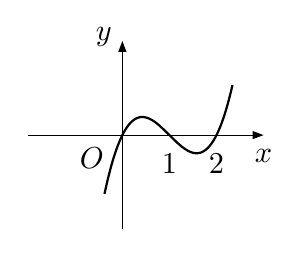
\begin{tikzpicture}[x=1pt, y=1pt,
    every node/.style={inner sep=0pt, font=\fontsize{10.5pt}{12.6pt}\selectfont}]
  % --- 坐标轴（轴身止于箭头底边，箭头为内容流中的独立填充三角形）
  \draw[line width=0.4pt] (-34.017,0) -- (47.438,0); % x 轴轴身
  \fill (51.025,0) -- (47.040,1.494) -- (47.040,-1.494) -- cycle; % x 箭头
  \draw[line width=0.4pt] (0,-34.017) -- (0,30.430); % y 轴轴身
  \fill (0,34.016) -- (1.494,30.031) -- (-1.494,30.031) -- cycle; % y 箭头
  % --- 三次函数曲线（内容流 299 段三次 Bézier → 0.02pt 容差 57 点折线）
  \draw[line width=0.8pt]
      (-6.463,-21.227) -- (-5.299,-16.066) -- (-4.112,-11.446) -- (-3.514,-9.357) -- (-2.894,-7.348) -- (-2.273,-5.498) --
      (-1.641,-3.772) -- (-1.020,-2.227) -- (-0.387,-0.801) -- (0.274,0.534) -- (0.936,1.721) -- (1.596,2.756) --
      (2.264,3.664) -- (2.954,4.458) -- (3.648,5.117) -- (4.364,5.656) -- (5.085,6.064) -- (5.809,6.343) --
      (6.573,6.507) -- (7.349,6.544) -- (8.125,6.460) -- (8.938,6.253) -- (9.783,5.921) -- (10.572,5.514) --
      (11.396,5.001) -- (12.266,4.374) -- (13.197,3.620) -- (15.059,1.923) -- (18.487,-1.468) -- (19.931,-2.837) --
      (21.408,-4.106) -- (22.104,-4.638) -- (22.791,-5.114) -- (23.581,-5.591) -- (24.343,-5.971) -- (25.065,-6.249) --
      (25.781,-6.439) -- (26.488,-6.535) -- (27.151,-6.536) -- (27.812,-6.445) -- (28.456,-6.262) -- (29.243,-5.904) --
      (30.019,-5.397) -- (30.784,-4.739) -- (31.549,-3.914) -- (32.286,-2.951) -- (33.006,-1.844) -- (33.721,-0.575) --
      (34.431,0.859) -- (35.118,2.422) -- (35.800,4.147) -- (36.490,6.077) -- (37.158,8.131) -- (37.817,10.340) --
      (38.494,12.801) -- (39.153,15.395) -- (39.785,18.071);
  % --- 标签
  \node at (-6.648,35.400) {$y$};
  \node at (-10.998,-8.250) {$O$};
  \node at (17.012,-10.240) {$1$};
  \node at (34.012,-10.240) {$2$};
  \node at (51.022,-7.390) {$x$};
\end{tikzpicture}
% ----------------------------------------------------------------------------
% 自验：轴端点 (−34.017,0)/(47.438,0) 与 (0,−34.017)/(0,30.430) 和内容流 574.5115/655.9662/582.4135/646.86 逐点吻合；曲线 57 点对源 Bézier 的最大偏差 < 0.02 pt；曲线与 x 轴交点 local x = −0.015 / 17.038 / 34.002，与标签 1、2 的横坐标 17.012 / 34.012 一致（偏差 < 0.03 pt）。标签净距（字形墨迹包围盒对路径中心线，已扣除线宽半宽）：y 3.30、O 2.14、1 4.00、2 2.41、x 2.95 pt，均 ≥ 2 pt。探针编译：xelatex 0 错误、0 警告。
% ============================================================================
\end{center}
\nopagebreak[4]
（A）$b \in (-\infty, 0)$　（B）$b \in (0, 1)$　（C）$b \in (1, 2)$　（D）$b \in (2, +\infty)$

\Needspace{4\baselineskip}
\textbf{解析}

图象左端 $x\to-\infty$ 时 $y\to-\infty$，右端 $x\to+\infty$ 时 $y\to+\infty$，故 $a>0$。
图象在 $x>0$ 内有一个极大值点和一个极小值点（分别位于 $(0,1)$ 与 $(1,2)$ 之间）。$f'(x)=3ax^2+2bx+c$ 的两根 $x_1,x_2$ 均为正，由韦达定理 $x_1+x_2=-\dfrac{2b}{3a}>0$，结合 $a>0$ 得 $b<0$。

验证：以 $f(x)=x(x-1)(x-2)=x^3-3x^2+2x$ 为例，$a=1>0$、$b=-3<0$、$c=2$，极值点 $x=1\pm\frac{1}{\sqrt3}\approx0.42,1.58$ 均在正半轴、零点为 $0,1,2$，图形与题图一致 。
（题图为示意图，$y$ 轴截距不可精确读取，但本题只需 $b$ 的符号，结论不受影响。）

\gkanswer{答案：A}

\end{answer}
\begin{answer}
\gksolhead{15}{}

\textbf{题目}：

函数 $y = \cos\left(\frac{2\pi}{3}x + \frac{\pi}{4}\right)$ 的最小正周期是\gkblank{}．

\Needspace{4\baselineskip}
\textbf{解析}

$y=\cos\!\left(\frac{2\pi}{3}x+\frac\pi4\right)$，$\omega=\frac{2\pi}{3}$，最小正周期 $T=\dfrac{2\pi}{\omega}=\dfrac{2\pi}{2\pi/3}=3$。

验证：$x=0$ 时相位 $\frac\pi4$；$x=3$ 时相位 $\frac{2\pi}{3}\cdot3+\frac\pi4=2\pi+\frac\pi4$，函数值相同 。

\gkanswer{答案：$3$。}

\end{answer}
\begin{answer}
\gksolhead{16}{}

\textbf{题目}：

已知一体积为 72 的正四面体，连结两个面的重心 $E$、$F$，则线段 $EF$ 的长是\gkblank{}．

\Needspace{4\baselineskip}
\textbf{解析}

设正四面体棱长为 $s$，体积 $V=\dfrac{\sqrt2}{12}s^3=72$，故 $s^3=432\sqrt2$。因 $(6\sqrt2)^3=216\cdot2\sqrt2=432\sqrt2$，得 $s=6\sqrt2$。
四面体任意两个面必共一条棱。设公共棱为 $AB$，第三顶点分别为 $C,D$，则两面重心 $E=\frac{A+B+C}{3}$，$F=\frac{A+B+D}{3}$，故 $\overrightarrow{EF}=\frac13\overrightarrow{CD}$，$EF=\frac{s}{3}=2\sqrt2$。

验证：$s=6\sqrt2$ 时 $V=\frac{\sqrt2}{12}(6\sqrt2)^3=\frac{\sqrt2}{12}\cdot432\sqrt2=\frac{864}{12}=72$ ；$EF=6\sqrt2/3=2\sqrt2\approx2.828$，小于棱长 $8.485$，合理 。因任意两面均共棱，答案与"取哪两个面"无关。

\gkanswer{答案：$2\sqrt2$。}

\end{answer}
\begin{answer}
\gksolhead{17}{}

\textbf{题目}：

$\left(\sqrt{x} - \frac{1}{\sqrt[3]{x}}\right)^{10}$ 展开式中的常数项是\gkblank{}．

\Needspace{4\baselineskip}
\textbf{解析}

通项 $T_{k+1}=\mathrm C_{10}^k(\sqrt x)^{10-k}\left(-\dfrac{1}{\sqrt[3]{x}}\right)^{k}=\mathrm C_{10}^k(-1)^k x^{\frac{10-k}{2}-\frac{k}{3}}$。
令指数为零：$3(10-k)-2k=0\Rightarrow k=6$。常数项 $=\mathrm C_{10}^6(-1)^6=210$。

验证：$k=6$ 时 $(\sqrt x)^4\cdot x^{-2}=x^2\cdot x^{-2}=1$ ，系数 $\mathrm C_{10}^6=210$ （$\mathrm C_{10}^4=210$ 亦同）。

\gkanswer{答案：$210$。}

\end{answer}
\begin{answer}
\gksolhead{18}{}

\textbf{题目}：

在空间，下列命题正确的是\gkblank{}．（注：把你认为正确的命题的序号都填上）

① 如果两直线 $a$、$b$ 分别与直线 $l$ 平行，那么 $a \parallel b$；

② 如果直线 $a$ 与平面 $\beta$ 内的一条直线 $b$ 平行，那么 $a \parallel \beta$；

③ 如果直线 $a$ 与平面 $\beta$ 内的两条直线 $b$、$c$ 都有垂直，那么 $a \perp \beta$；

④ 如果平面 $\beta$ 内的一条直线 $a$ 垂直平面 $\gamma$，那么 $\beta \perp \gamma$．

\Needspace{4\baselineskip}
\textbf{解析}

① 平行于同一条直线的两条直线互相平行（公理 4），\textbf{正确}。
② 若 $a\subset\beta$，则 $a$ 与 $\beta$ 内某直线平行却 $a\not\parallel\beta$，缺少 $a\not\subset\beta$ 的条件，\textbf{错误}。
③ 需 $b,c$ 相交；若 $b\parallel c$，$a$ 可同时垂直 $b,c$ 而不垂直于 $\beta$，\textbf{错误}。
④ $a\subset\beta$ 且 $a\perp\gamma$，由面面垂直的判定定理得 $\beta\perp\gamma$，\textbf{正确}。

验证：② 取 $\beta:z=0$，$a$ 为 $\beta$ 内直线，$b$ 为 $\beta$ 内与 $a$ 平行的直线，条件满足但 $a\subset\beta$ ；③ 取 $\beta:z=0$，$b,c$ 均平行于 $x$ 轴，$a$ 取 $y$ 轴方向，则 $a\perp b$、$a\perp c$ 但 $a\subset\beta$，不垂直 $\beta$ 。故只有 ①④。

\gkanswer{答案：①④。}

\end{answer}
\begin{answer}
\gksolhead{19}{}

\textbf{题目}：

已知二次函数 $f(x) = (\lg a)x^2 + 2x + 4\lg a$ 的最大值为 3，求 $a$ 的值．

\Needspace{4\baselineskip}
\textbf{解析}

有最大值要求二次项系数 $\lg a<0$，即 $0<a<1$。
$f(x)=\lg a\left(x+\frac{1}{\lg a}\right)^2+4\lg a-\frac{1}{\lg a}$，最大值 $=4\lg a-\frac{1}{\lg a}=3$。
令 $t=\lg a<0$：$4t-\frac1t=3\Rightarrow4t^2-3t-1=0\Rightarrow t=1$ 或 $t=-\frac14$。取 $t=-\frac14$，故 $a=10^{-1/4}$。

验证：$a=10^{-1/4}$ 时 $f(x)=-\frac14x^2+2x-1$，顶点 $x=4$，$f(4)=-4+8-1=3$ ，且 $-\frac14<0$ 保证是最大值 。

\gkanswer{答案：$a=10^{-\frac14}$（即 $\dfrac{1}{\sqrt[4]{10}}$）。}

\end{answer}
\begin{answer}
\gksolhead{20}{}

\textbf{题目}：

在 $\triangle ABC$ 中，角 $A$、$B$、$C$ 对边分别为 $a$、$b$、$c$，证明：$\dfrac{a^2 - b^2}{c^2} = \dfrac{\sin(A - B)}{\sin C}$．

\Needspace{4\baselineskip}
\textbf{解析}

\Needspace{5\baselineskip}
由正弦定理 $a=2R\sin A,\ b=2R\sin B,\ c=2R\sin C$，
\nopagebreak[4]
\[\frac{a^2-b^2}{c^2}=\frac{\sin^2A-\sin^2B}{\sin^2C}.\]
\Needspace{5\baselineskip}
又 $\sin^2A-\sin^2B=\sin(A+B)\sin(A-B)$，而 $\sin(A+B)=\sin(\pi-C)=\sin C$，故
\nopagebreak[4]
\[\frac{a^2-b^2}{c^2}=\frac{\sin C\cdot\sin(A-B)}{\sin^2C}=\frac{\sin(A-B)}{\sin C}.\]

验证：取 $a=3,b=4,c=5$（$C=90^\circ$）：左 $=\frac{9-16}{25}=-\frac{7}{25}$；$\sin(A-B)=\frac35\cdot\frac35-\frac45\cdot\frac45=\frac{9-16}{25}=-\frac{7}{25}=$ 右 。

\gkanswer{答案：恒等式成立，证明见解析。}

\end{answer}
\begin{answer}
\gksolhead{21}{}

\textbf{题目}：

在直角梯形 $ABCD$ 中，$\angle D = \angle BAD = 90^\circ$，$AD = DC = \frac{1}{2}AB = a$（如图一）．将 $\triangle ADC$ 沿 $AC$ 折起，使 $D$ 到 $D'$．记面 $ACD'$ 为 $\alpha$，面 $ABC$ 为 $\beta$，面 $BCD'$ 为 $\gamma$．

（1） 若二面角 $\alpha-AC-\beta$ 为直二面角（如图二），求二面角 $\beta-BC-\gamma$ 的大小；

（2） 若二面角 $\alpha-AC-\beta$ 为 $60^\circ$（如图三），求三棱锥 $D'-ABC$ 的体积．
\nopagebreak[4]
\begin{center}% ============================================================================
% 2000 年春季高考（京、皖）文科 第 21 题 图一：直角梯形 ABCD
% ----------------------------------------------------------------------------
% 来源：.work/phase4-b20/source/2000春季京皖文.pdf
%       SHA-256 b9552b8354735296f6ea1ed051085e094e4af0c14ff97ada2dbd4e579b14287f
%       第 1 页，内容流对象 47（图注「图一」为排版文字，不在本图内）
% 重绘方式：qpdf --qdf 取内容流 → 解析 m/l/c/re/S/f、w、d → 本地坐标
%          本地坐标 = 页面坐标 − (874.160, 359.960)，原点取顶点 A（梯形左下角）；
%          1 单位 = 1 TeX pt；页面为 A3（1190.55 × 841.89 pt）。
% 元素计数：实线路径 4（AB、BC、CD、DA），虚线路径 1（AC），标签 4（A, B, C, D）
% 线宽：全部 0.40 pt；虚线 on/off 各 2.99 pt
% 坐标基准与源位的偏差：端点四舍五入到 0.001 pt；全部为直线段，无简化。
% 标签：位置 = pdftotext -bbox 文本中心 − 基准；D 源位 (−5.070,37.990)，左移 1.6 pt；C 源位 (38.580,37.990)，右移 1.0 pt、上移 2.2 pt；A、B 未动。净距均 ≥ 2 pt
% ============================================================================
\begin{tikzpicture}[x=1pt, y=1pt,
    every node/.style={inner sep=0pt, font=\fontsize{10.5pt}{12.6pt}\selectfont}]
  % --- 实线：AB、BC、CD、DA（内容流顺序为 AB→BC→CD→DA）
  \draw[line width=0.4pt] (0,0) -- (68.040,0);
  \draw[line width=0.4pt] (68.040,0) -- (34.020,34.020);
  \draw[line width=0.4pt] (34.020,34.020) -- (0,34.020);
  \draw[line width=0.4pt] (0,34.020) -- (0,0);
  % --- 虚线：AC（划长 2.99 pt，内容流 [2.98883 2.98883] 0 d）
  \draw[line width=0.4pt, dash pattern=on 2.99pt off 2.99pt] (0,0) -- (34.020,34.020);
  % --- 标签
  \node at (-6.670,37.990) {$D$};
  \node at (39.580,40.190) {$C$};
  \node at (-4.930,-5.890) {$A$};
  \node at (72.710,-5.890) {$B$};
  % 图注（源页图下居中；主会话添加）
  \node at (34.020,-12.000) {图一};
\end{tikzpicture}
% ----------------------------------------------------------------------------
% 自验：A=(0,0)、B=(68.040,0)、C=(34.020,34.020)、D=(0,34.020)，与内容流 874.16/942.20/908.18/874.16、359.96/393.98 逐点吻合；AD=DC=34.020、AB=68.040，满足题设 AD=DC=½AB；标签：A、B 取源位；D 左移 1.6 pt、C 右移 1.0 pt 并上移 2.2 pt。净距 A 3.32、B 3.22、D 2.44、C 2.18 pt。探针编译：0 错误、0 警告。
% ============================================================================
\end{center}
\nopagebreak[4]
\nopagebreak[4]
\begin{center}% ============================================================================
% 2000 年春季高考（京、皖）文科 第 21 题 图二：折叠后三棱锥 D′-ABC（直二面角）
% ----------------------------------------------------------------------------
% 来源：.work/phase4-b20/source/2000春季京皖文.pdf
%       SHA-256 b9552b8354735296f6ea1ed051085e094e4af0c14ff97ada2dbd4e579b14287f
%       第 1 页，内容流对象 47（图注「图二」不在本图内）
% 重绘方式：qpdf --qdf 取内容流 → 解析 m/l/c/re/S/f、w、d → 本地坐标
%          本地坐标 = 页面坐标 − (970.740, 359.960)，原点取顶点 A；
%          1 单位 = 1 TeX pt；页面为 A3（1190.55 × 841.89 pt）。
% 元素计数：实线路径 3（AB、BD′、D′A），虚线路径 3（AC、BC、CD′），标签 4（A, B, C, D′）
% 线宽：全部 0.40 pt；虚线 on/off 各 2.99 pt
% 坐标基准与源位的偏差：端点四舍五入到 0.001 pt；全部为直线段，无简化。
% 标签：位置 = pdftotext -bbox 文本中心 − 基准；C、D′ 取「字母 + 撇」合成包围盒中心（撇号在内容流中为独立 F9 字形，pdftotext 未单列）；C 源位 (21.920,14.130)，右移 2.4 pt、下移 3.4 pt；其余未动。净距均 ≥ 2 pt
% ============================================================================
\begin{tikzpicture}[x=1pt, y=1pt,
    every node/.style={inner sep=0pt, font=\fontsize{10.5pt}{12.6pt}\selectfont}]
  % --- 实线：AB、BD′、D′A
  \draw[line width=0.4pt] (0,0) -- (68.040,0);
  \draw[line width=0.4pt] (68.040,0) -- (17.010,34.020);
  \draw[line width=0.4pt] (17.010,34.020) -- (0,0);
  % --- 虚线：AC、BC、CD′
  \draw[line width=0.4pt, dash pattern=on 2.99pt off 2.99pt] (0,0) -- (20.410,20.410);
  \draw[line width=0.4pt, dash pattern=on 2.99pt off 2.99pt] (68.040,0) -- (20.410,20.410);
  \draw[line width=0.4pt, dash pattern=on 2.99pt off 2.99pt] (20.410,20.410) -- (17.010,34.020);
  % --- 标签
  \node at (-4.930,-5.890) {$A$};
  \node at (72.710,-5.890) {$B$};
  \node at (16.760,41.350) {$D'$};
  \node at (24.320,10.730) {$C$};
  % 图注（源页图下居中；主会话添加）
  \node at (34.020,-12.000) {图二};
\end{tikzpicture}
% ----------------------------------------------------------------------------
% 自验：A=(0,0)、B=(68.040,0)、D′=(17.010,34.020)、C=(20.410,20.410)，与内容流 970.74/1038.78/987.75/991.15、359.96/393.98/380.37 逐点吻合；D′ 到 A、B 的距离分别 38.03、61.33 pt，C 由三条虚线汇于一点；标签：A、B、D′ 取源位；C 合成中心 (992.66,374.09) 右移 2.4 pt、下移 3.4 pt。净距 A 3.31、B 3.23、D′ 3.71、C 2.26 pt。探针编译：0 错误、0 警告。
% ============================================================================
\end{center}
\nopagebreak[4]
\nopagebreak[4]
\begin{center}% ============================================================================
% 2000 年春季高考（京、皖）文科 第 21 题 图三：折叠后三棱锥 D′-ABC（二面角 60°）
% ----------------------------------------------------------------------------
% 来源：.work/phase4-b20/source/2000春季京皖文.pdf
%       SHA-256 b9552b8354735296f6ea1ed051085e094e4af0c14ff97ada2dbd4e579b14287f
%       第 1 页，内容流对象 47（图注「图三」不在本图内）
% 重绘方式：qpdf --qdf 取内容流 → 解析 m/l/c/re/S/f、w、d → 本地坐标
%          本地坐标 = 页面坐标 − (1067.320, 359.960)，原点取顶点 A；
%          1 单位 = 1 TeX pt；页面为 A3（1190.55 × 841.89 pt）。
% 元素计数：实线路径 3（AB、BD′、D′A），虚线路径 3（AC、BC、CD′），标签 4（A, B, C, D′）
% 线宽：全部 0.40 pt；虚线 on/off 各 2.99 pt
% 坐标基准与源位的偏差：端点四舍五入到 0.001 pt；全部为直线段，无简化。
% 标签：位置 = pdftotext -bbox 文本中心 − 基准；C、D′ 取「字母 + 撇」合成包围盒中心（撇号在内容流中为独立 F9 字形，pdftotext 未单列）；C 源位 (21.930,14.125)，右移 2.4 pt、下移 3.4 pt；其余未动。净距均 ≥ 2 pt
% ============================================================================
\begin{tikzpicture}[x=1pt, y=1pt,
    every node/.style={inner sep=0pt, font=\fontsize{10.5pt}{12.6pt}\selectfont}]
  % --- 实线：AB、BD′、D′A
  \draw[line width=0.4pt] (0,0) -- (68.040,0);
  \draw[line width=0.4pt] (68.040,0) -- (25.510,34.020);
  \draw[line width=0.4pt] (25.510,34.020) -- (0,0);
  % --- 虚线：AC、BC、CD′
  \draw[line width=0.4pt, dash pattern=on 2.99pt off 2.99pt] (0,0) -- (20.410,20.410);
  \draw[line width=0.4pt, dash pattern=on 2.99pt off 2.99pt] (68.040,0) -- (20.410,20.410);
  \draw[line width=0.4pt, dash pattern=on 2.99pt off 2.99pt] (20.410,20.410) -- (25.510,34.020);
  % --- 标签
  \node at (-4.930,-5.890) {$A$};
  \node at (72.700,-5.890) {$B$};
  \node at (25.265,41.350) {$D'$};
  \node at (24.330,10.725) {$C$};
  % 图注（源页图下居中；主会话添加）
  \node at (34.020,-12.000) {图三};
\end{tikzpicture}
% ----------------------------------------------------------------------------
% 自验：A=(0,0)、B=(68.040,0)、D′=(25.510,34.020)、C=(20.410,20.410)，与内容流 1067.32/1135.36/1092.83/1087.73、359.96/393.98/380.37 逐点吻合；D′ 的横坐标较图二右移 8.50 pt（60° 情形），C 位置与图二相同；标签合成中心 D′=(1092.585,401.31)、C=(1089.25,374.09)，换算后为 (25.265,41.350)、(21.930,14.125)；C 另右移 2.4 pt、下移 3.4 pt。净距 A 3.30、B 3.23、D′ 3.71、C 2.25 pt。探针编译：0 错误、0 警告。
% ============================================================================
\end{center}
\nopagebreak[4]
\Needspace{4\baselineskip}
\textbf{解析}

折起前建系：$A(0,0,0)$、$B(2a,0,0)$、$C(a,a,0)$、$D(0,a,0)$（此时 $AD=DC=a$，$AB=2a$，$\angle A=\angle D=90^\circ$）。
\Needspace{5\baselineskip}
取 $AC$ 中点 $M\left(\frac a2,\frac a2,0\right)$，$|MD|=\frac{|AC|}{2}=\frac{a\sqrt2}{2}=\frac{a}{\sqrt2}$（直角三角形 $ADC$ 斜边中线）。记 $u=\left(-\frac{1}{\sqrt2},\frac{1}{\sqrt2},0\right)$ 为平面 $ABC$ 内垂直 $AC$、指向 $D$ 一侧的单位向量，$v=(0,0,1)$。含 $B$ 的半平面位于 $-u$ 一侧，故以题设内二面角 $\theta$ 为参数，折起后
\nopagebreak[4]
\[D'=M+\frac{a}{\sqrt2}\left(-\cos\theta\,u+\sin\theta\,v\right),\quad \theta=\text{\text{二面角} }\alpha-AC-\beta .\]

\gksubpart{(1)}

$\theta=90^\circ$：$D'\left(\frac a2,\frac a2,\frac{\sqrt2}{2}a\right)$。
求 $\beta-BC-\gamma$：取 $BC$ 方向 $d=\left(-\frac{1}{\sqrt2},\frac{1}{\sqrt2},0\right)$。
在面 $\beta=ABC$ 内：$\overrightarrow{BA}=(-2a,0,0)$，$\overrightarrow{BA}\cdot d=\sqrt2a$，得垂直分量为 $(-a,-a,0)$，单位化 $p_1=\left(-\frac{1}{\sqrt2},-\frac{1}{\sqrt2},0\right)$。
在面 $\gamma=BCD'$ 内：$\overrightarrow{BD'}=\left(-\frac{3a}{2},\frac a2,\frac{\sqrt2a}{2}\right)$，$\overrightarrow{BD'}\cdot d=\sqrt2a$，垂直分量为 $\left(-\frac a2,-\frac a2,\frac{\sqrt2a}{2}\right)$，模为 $a$，单位化 $p_2=\left(-\frac12,-\frac12,\frac{\sqrt2}{2}\right)$。
$\cos\langle p_1,p_2\rangle=\frac{1}{\sqrt2}$，故二面角为 $45^\circ$。

\gksubpart{(2)}

$\theta=60^\circ$：$D'=\left(\frac{3a}{4},\frac a4,\frac{\sqrt6}{4}a\right)$，到平面 $ABC$ 的距离 $h=\frac{a}{\sqrt2}\sin60^\circ=\frac{\sqrt6}{4}a$。
\Needspace{5\baselineskip}
$S_{\triangle ABC}=\frac12\cdot2a\cdot a=a^2$，故
\nopagebreak[4]
\[V=\frac13\cdot a^2\cdot\frac{\sqrt6}{4}a=\frac{\sqrt6}{12}a^3 .\]

验证：取 $a=1$。(1) 用体积法：$S_{\triangle ABC}=1$，$S_{\triangle BCD'}=\frac12|\overrightarrow{BC}\times\overrightarrow{BD'}|=\frac{\sqrt2}{2}$，$|BC|=\sqrt2$，$V=\frac13\cdot1\cdot\frac{\sqrt2}{2}=0.2357$；由 $3V|BC|=2S_1S_2\sin\varphi$ 得 $\sin\varphi=\frac{3(0.2357)(1.4142)}{2(1)(0.7071)}=0.7071$，$\varphi=45^\circ$ 。
(2) 数值代入 $\frac{\sqrt6}{12}=0.2041$，与 $\frac13\cdot1\cdot\frac{\sqrt6}{4}$ 相同 。

\gkanswer{答案（1）：$45^\circ$}

\gkanswer{答案（2）：$V_{D'-ABC}=\dfrac{\sqrt6}{12}a^3$}

\end{answer}
\begin{answer}
\gksolhead{22}{}

\textbf{题目}：

已知等差数列 $\{a_n\}$ 的公差和等比数列 $\{b_n\}$ 的公比相等，且都等于 $d$（$d > 0$，$d \neq 1$），若 $a_1 = b_1$，$a_3 = 3b_3$，$a_5 = 5b_5$，求 $a_n$，$b_n$．

\Needspace{4\baselineskip}
\textbf{解析}

\Needspace{5\baselineskip}
设 $a_1=b_1=c$，公差、公比同为 $d>0,\ d\ne1$。
\nopagebreak[4]
\[a_3=c+2d=3b_3=3cd^2,\qquad a_5=c+4d=5b_5=5cd^4 .\]
\Needspace{5\baselineskip}
即 $2c(3d^2-1)=4d=c(5d^4-1)$，故 $c\,(5d^4-6d^2+1)=0$。因 $c=0$ 会使 $2d=0$ 与 $d>0$ 矛盾，故 $c\ne0$，从而
\nopagebreak[4]
\[5d^4-6d^2+1=0\Rightarrow(d^2-1)(5d^2-1)=0 .\]
由 $d\ne1,\ d>0$ 得 $d=\frac{1}{\sqrt5}=\frac{\sqrt5}{5}$。代回 $c=\dfrac{2d}{3d^2-1}=\dfrac{2/\sqrt5}{3/5-1}=-\sqrt5$。
故 $a_n=-\sqrt5+(n-1)\dfrac{\sqrt5}{5}=\dfrac{\sqrt5}{5}(n-6)$，$b_n=-\sqrt5\left(\dfrac{\sqrt5}{5}\right)^{n-1}$。

验证：$a_3=-\sqrt5+\frac{2\sqrt5}{5}=-\frac{3\sqrt5}{5}$，$b_3=-\frac{\sqrt5}{5}$，$3b_3=-\frac{3\sqrt5}{5}=a_3$ ；$a_5=-\frac{\sqrt5}{5}$，$b_5=-\frac{\sqrt5}{25}$，$5b_5=-\frac{\sqrt5}{5}=a_5$ ；$a_1=b_1=-\sqrt5$ 。

\gkanswer{答案：$a_n=\dfrac{\sqrt5}{5}(n-6)$，$b_n=-\sqrt5\left(\dfrac{\sqrt5}{5}\right)^{n-1}$（即 $b_n=-(\sqrt5)^{\,2-n}$）。}

\end{answer}
\begin{answer}
\gksolhead{23}{}

\textbf{题目}：

如图，设点 $A$ 和 $B$ 为抛物线 $y^2 = 4px$（$p > 0$）上原点以外的两个动点，已知 $OA \perp OB$，$OM \perp AB$．求点 $M$ 的轨迹方程，并说明它表示什么曲线．
\nopagebreak[4]
\begin{center}% ============================================================================
% 2000 年春季高考（京、皖）文科 第 23 题：抛物线 y² = 4px 与点 A、B、M
% ----------------------------------------------------------------------------
% 来源：.work/phase4-b20/source/2000春季京皖文.pdf
%       SHA-256 b9552b8354735296f6ea1ed051085e094e4af0c14ff97ada2dbd4e579b14287f
%       第 2 页，内容流对象 2
% 重绘方式：qpdf --qdf 取内容流 → 解析 m/l/c/re/S/f、w、d → 本地坐标
%          本地坐标 = 页面坐标 − (701.132, 687.581)，原点取坐标原点 O；
%          1 单位 = 1 TeX pt；页面为 A3（1190.55 × 841.89 pt）。
% 元素计数：实线路径 8（x 轴、y 轴、抛物线上支、下支、OA、OB、AB、OM），填充箭头 2，虚线 0，标签 6（O, A, B, M, x, y）
% 线宽：轴与辅助线 0.40 pt；抛物线两支 0.80 pt（内容流 w=0.79701）；箭头填充三角形长 3.99 pt、半宽 1.49 pt
% 坐标基准与源位的偏差：端点四舍五入到 0.001 pt；抛物线两支按 24 段三次 Bézier 采样的折线重绘，经 0.02 pt 容差简化（每支 32 点），最大偏差 < 0.02 pt。
% 标签：位置 = pdftotext -bbox 文本中心 − 基准；O、A、B、M、y 未动；x 源位 (68.578,−5.591)，下移 1.6 pt。净距均 ≥ 2 pt
% ============================================================================
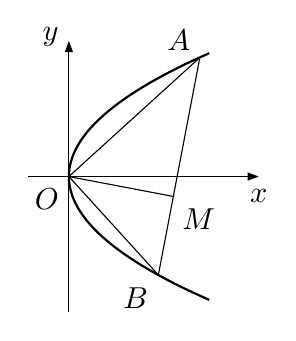
\begin{tikzpicture}[x=1pt, y=1pt,
    every node/.style={inner sep=0pt, font=\fontsize{10.5pt}{12.6pt}\selectfont}]
  % --- 坐标轴（轴身止于箭头底边，箭头为独立填充三角形）
  \draw[line width=0.4pt] (-14.695,0) -- (64.989,0); % x 轴轴身
  \fill (68.576,0) -- (64.591,1.494) -- (64.591,-1.494) -- cycle; % x 箭头
  \draw[line width=0.4pt] (0,-48.983) -- (0,45.396); % y 轴轴身
  \fill (0,48.983) -- (1.494,44.998) -- (-1.494,44.998) -- cycle; % y 箭头
  % --- 抛物线 y^2=4px 上、下两支（内容流 24 段三次 Bézier → 0.02pt 容差 32 点折线）
  \draw[line width=0.8pt]
      (0.000,0.000) -- (0.076,1.712) -- (0.202,2.786) -- (0.408,3.995) -- (0.792,5.572) -- (1.305,7.148) --
      (1.786,8.357) -- (2.337,9.567) -- (3.169,11.143) -- (4.130,12.720) -- (4.955,13.929) -- (5.849,15.138) --
      (7.129,16.715) -- (8.539,18.291) -- (9.708,19.500) -- (10.946,20.710) -- (12.675,22.286) -- (14.532,23.863) --
      (16.045,25.072) -- (17.627,26.281) -- (19.804,27.858) -- (22.110,29.434) -- (23.967,30.644) -- (25.893,31.853) --
      (28.518,33.429) -- (31.272,35.006) -- (33.473,36.215) -- (35.743,37.424) -- (38.816,39.001) -- (42.019,40.577) --
      (44.563,41.787) -- (50.699,44.572);
  \draw[line width=0.8pt]
      (0.000,0.000) -- (0.076,-1.712) -- (0.202,-2.786) -- (0.408,-3.995) -- (0.792,-5.572) -- (1.305,-7.148) --
      (1.786,-8.357) -- (2.337,-9.567) -- (3.169,-11.143) -- (4.130,-12.720) -- (4.955,-13.929) -- (5.849,-15.138) --
      (7.129,-16.715) -- (8.539,-18.291) -- (9.708,-19.500) -- (10.946,-20.710) -- (12.675,-22.286) -- (14.532,-23.863) --
      (16.045,-25.072) -- (17.627,-26.281) -- (19.804,-27.858) -- (22.110,-29.434) -- (23.967,-30.644) -- (25.893,-31.853) --
      (28.518,-33.429) -- (31.272,-35.006) -- (33.473,-36.215) -- (35.743,-37.424) -- (38.816,-39.001) -- (42.019,-40.577) --
      (44.563,-41.787) -- (50.699,-44.572);
  % --- 辅助线：OA、OB、AB、OM
  \draw[line width=0.4pt] (0,0) -- (47.317,43.007);   % OA
  \draw[line width=0.4pt] (0,0) -- (32.329,-35.562);  % OB
  \draw[line width=0.4pt] (32.329,-35.562) -- (47.317,43.007); % AB
  \draw[line width=0.4pt] (0,0) -- (38.108,-7.270);   % OM ⊥ AB
  % --- 标签
  \node at (-7.990,-8.250) {$O$};
  \node at (39.680,49.330) {$A$};
  \node at (24.120,-43.810) {$B$};
  \node at (46.900,-15.520) {$M$};
  \node at (68.580,-7.190) {$x$};
  \node at (-6.650,50.370) {$y$};
\end{tikzpicture}
% ----------------------------------------------------------------------------
% 自验：A=(47.317,43.007) 即页面 (748.449,730.588)、B=(32.329,−35.562) 即 (733.460,652.020)、M=(38.108,−7.270) 即 (739.240,680.311)，均在内容流端点 0.001 pt 内；OA·OB = 0.0（OA⊥OB），OM·AB = 0.0（OM⊥AB，|OM| = 38.795 pt）；两支对 x = 0.025521·y² 的最大残差 0.012 pt（y² = 4px，p ≈ 9.80 pt），两支端点 (50.699,±44.572) 与源 (751.831,732.153)/(751.831,643.009) 吻合。标签：O、A、B、M、y 取源位，x 下移 1.6 pt；净距 O 3.89、A 2.41、B 6.58、M 5.11、x 2.98、y 3.44 pt。探针编译：0 错误、0 警告。
% ============================================================================
\end{center}
\nopagebreak[4]
\Needspace{4\baselineskip}
\textbf{解析}

设 $A(pt_1^2,2pt_1)$、$B(pt_2^2,2pt_2)$（$t_1,t_2\ne0$，且 $A\ne B$）。
$OA\perp OB\Rightarrow p^2t_1^2t_2^2+4p^2t_1t_2=0\Rightarrow t_1t_2=-4$。
弦 $AB$：$y(t_1+t_2)=2x+2pt_1t_2$，即 $2x-(t_1+t_2)y-8p=0$。记 $k=t_1+t_2$（由 $t_1t_2=-4$ 知 $k$ 可取任意实数）。
\Needspace{5\baselineskip}
$M$ 是 $O$ 到 $AB$ 的垂足，由点到直线公式
\nopagebreak[4]
\[M=\frac{8p\,(2,\,-k)}{4+k^2},\quad\text{\text{即} } x=\frac{16p}{4+k^2},\ y=-\frac{8pk}{4+k^2}.\]
消去 $k$：$x^2+y^2=\frac{64p^2(4+k^2)}{(4+k^2)^2}=\frac{64p^2}{4+k^2}=4p\cdot\frac{16p}{4+k^2}=4px$。
因 $x=\frac{16p}{4+k^2}>0$，原点 $(0,0)$ 不在轨迹上（但为极限点）。

验证：取 $p=1,t_1=1,t_2=-4$：$A(1,2)$、$B(16,-8)$，$\overrightarrow{OA}\cdot\overrightarrow{OB}=16-16=0$ ；$AB:2x+3y-8=0$，垂足 $M\left(\frac{16}{13},\frac{24}{13}\right)$，代入 $x^2+y^2-4x=\frac{832}{169}-\frac{832}{169}=0$ 。另随机多组参数数值验证，均满足轨迹方程且 $M$ 在 $AB$ 上。

\gkanswer{答案：轨迹方程为 $x^2+y^2=4px\ (x\ne0)$；它表示以 $(2p,0)$ 为圆心、$2p$ 为半径的圆，但除去原点 $O$。}

\end{answer}
\begin{answer}
\gksolhead{24}{}

\textbf{题目}：

某地区上年度电价为 $0.8$ 元/kW$\cdot$h，年用电量为 $a$ kW$\cdot$h　本年度计划将电价降到 $0.55$ 元/kW$\cdot$h 至 $0.75$ 元/kW$\cdot$h 之间，而用户期望电价为 $0.4$ 元/kW$\cdot$h　经测算，下调电价后新增的用电量与实际电价和用户期望电价的差成反比（比例系数为 $k$）．该地区电力的成本为 $0.3$ 元/kW$\cdot$h．

（1） 写出本年度电价下调后，电力部门的收益 $y$ 与实际电价 $x$ 的函数关系式；

（2） 设 $k = 0.2a$，当电价最低定为多少时仍可保证电力部门的收益比上年至少增长 $20\%$？

注：收益 = 实际用电量 ×（实际电价 $-$ 成本价）

\Needspace{4\baselineskip}
\textbf{解析}

\gksubpart{(1)}

\Needspace{5\baselineskip}
新增用电量 $=\dfrac{k}{x-0.4}$，总用电量 $=a+\dfrac{k}{x-0.4}$，故收益
\nopagebreak[4]
\[y=\left(a+\frac{k}{x-0.4}\right)(x-0.3),\qquad x\in[0.55,\,0.75].\]
\gksubpart{(2)}

上年收益 $=a(0.8-0.3)=0.5a$，要求 $y\ge1.2\times0.5a=0.6a$。
\Needspace{5\baselineskip}
取 $k=0.2a$：$\left(1+\dfrac{0.2}{x-0.4}\right)(x-0.3)\ge0.6$。令 $u=x-0.4\in[0.15,0.35]$，则 $x-0.3=u+0.1$：
\nopagebreak[4]
\[u+0.1+0.2\cdot\frac{u+0.1}{u}\ge0.6\iff u+0.3+\frac{0.02}{u}\ge0.6,\]
\nopagebreak[4]
\[\iff u^2-0.3u+0.02\ge0\iff(u-0.1)(u-0.2)\ge0.\]
在 $u\in[0.15,0.35]$ 内须 $u\ge0.2$，即 $x\ge0.6$。故最低电价为 $0.6$ 元/(kW·h)。

验证：$x=0.6$：用电 $a+\frac{0.2a}{0.2}=2a$，收益 $2a\times0.3=0.6a=1.2\times0.5a$ （恰好增长 20\%）；$x=0.58$：收益 $a(1+\frac{0.2}{0.18})(0.28)\approx0.591a<0.6a$ ；$x=0.75$：$a(1+\frac{0.2}{0.35})(0.45)\approx0.707a\ge0.6a$ 。临界值确为 $0.6$。

\gkanswer{答案（1）：$y=\left(a+\dfrac{k}{x-0.4}\right)(x-0.3)$，$0.55\le x\le0.75$}

\gkanswer{答案（2）：电价最低定为 $0.6$ 元/(kW·h)}

\par\medskip

\end{answer}